\chapter{Modelli e disegno sperimentale}
\label{chap:modelli}

Il protocollo del \cref{chap:dataset} mantiene controllati gli oggetti
utilizzati per addestramento e valutazione. Su questa base, il presente
capitolo definisce che cosa viene modificato nel passaggio dal modello
classico a quello quantistico e quali condizioni rimangono invariate.
La domanda non è se una rete contenente un circuito quantistico possa
classificare immagini, ma se quel circuito apporti un beneficio rispetto
a un controllo classico che attraversa lo stesso collo di bottiglia.

\section{Impostazione del confronto}
\label{sec:disegno-confronto}

\subsection{Una rappresentazione classica comune}

Tutti i modelli ricevono un vettore \(\boldsymbol{f}\in\mathbb{R}^{512}\)
prodotto dalla stessa ResNet18 congelata, secondo il preprocessing e la
procedura di caching già descritti. Non viene effettuato un fine-tuning
del backbone sul dataset galattico. I parametri ottimizzati appartengono
esclusivamente alla testa di classificazione.

Il \cref{lst:feature-backbone} mostra la costruzione dell'estrattore
in \texttt{models/classical.py}. La sostituzione di \texttt{fc}
con l'identità restituisce le 512 feature invece dei logit ImageNet.
Durante il caching, \texttt{data/features.py} pone l'estrattore in
modalità \texttt{eval()} ed esegue l'inferenza entro
\texttt{torch.no\_grad()}. Le teste sono poi addestrate sulle feature
salvate: il backbone non appartiene al loro grafo di ottimizzazione.

\begin{code}
\begin{minted}{python}
def resnet18_backbone(*, pretrained: bool = True) -> nn.Module:
    weights = models.ResNet18_Weights.IMAGENET1K_V1 if pretrained else None
    backbone = models.resnet18(weights=weights)
    backbone.fc = nn.Identity()
    return backbone
\end{minted}
\caption{Costruzione della ResNet18 usata per il caching delle feature;
negli esperimenti viene selezionato \texttt{pretrained=True}.}
\label{lst:feature-backbone}
\end{code}

L'architettura ibrida segue il paradigma del \emph{dressed quantum
circuit}: una trasformazione classica prepara l'input del circuito e
un'altra ne converte l'uscita nei punteggi di classe. Mari et al.
\cite{mari2020transfer} hanno proposto questo schema nell'ambito del
transfer learning classico-quantistico. Nel telerilevamento, Otgonbaatar
et al.~\cite{otgonbaatar2023transfer} hanno studiato un'impostazione
basata su feature classiche e piccoli circuiti, considerando anche
varianti con data re-uploading. Questi lavori motivano il tipo di
architettura, non garantiscono un miglioramento nel diverso problema
affrontato qui.

Il modello della tesi non applica convoluzioni quantistiche ai pixel e
non include operazioni di pooling quantistico. È quindi distinto dalle
QCNN con strati di convoluzione e pooling, come quelle considerate da
Kim et al.~\cite{kim2023transfer}: la parte convoluzionale rimane
interamente classica.

\subsection{Ruolo delle famiglie di modelli}

Le baseline B0 e B1 forniscono due riferimenti contestuali: una testa
lineare e un percettrone multistrato. Il confronto centrale riguarda
invece B2, Q e QF. B2 è una testa classica con bottleneck di quattro o
otto componenti; Q inserisce, dopo la stessa compressione, un circuito
variazionale addestrabile; QF mantiene identico il circuito, ma ne
congela i parametri interni.

Questa separazione permette di distinguere tre domande. B0 e B1
indicano quanto le feature siano sfruttabili da classificatori classici.
Il confronto Q--B2 valuta l'inserimento del circuito a parità di
dimensione del bottleneck. Il confronto Q--QF studia il contributo
dell'ottimizzazione dei pesi circuitali, rispetto a una trasformazione
quantistica fissata all'inizializzazione. La \cref{fig:pipeline-modelli}
riassume la struttura del confronto principale.

\begin{figure}[tbp]
\centering
% Schema originale della struttura implementata: nessuna figura di articoli copiata.
\begin{tikzpicture}[
  font=\footnotesize,
  block/.style={draw=black!50,rounded corners=2pt,align=center,
    minimum height=0.95cm,text width=2.15cm,inner sep=4pt},
  flow/.style={-{Latex[length=2mm]},draw=black!55,line width=0.65pt}
]
\node[block,fill=black!3] (features) at (0,0)
  {ResNet18 congelata\\feature \(\boldsymbol f\in\mathbb R^{512}\)};
\foreach \row/\modelname/\yy in {b/B2/2,q/Q/0,f/QF/-2}{
  \node[block] (pre\row) at (3.1,\yy)
    {Proiezione + \(\pi\tanh\)\\\(512\rightarrow q\)};
  \node[anchor=south,yshift=2pt,font=\footnotesize\bfseries] at (pre\row.north) {\modelname};
  \node[block] (post\row) at (9.5,\yy)
    {Classificatore affine\\\(q\rightarrow K\)};
  \draw[flow] (features.east) -- (pre\row.west);
}
\node[block,fill=blue!5] (midb) at (6.3,2)
  {Nessun circuito\\Uscita: \(\boldsymbol a\)};
\node[block,fill=violet!7] (midq) at (6.3,0)
  {Circuito \(+\langle Z\rangle\)\\\(\boldsymbol\theta\) addestrabile};
\node[block,fill=orange!9] (midf) at (6.3,-2)
  {Circuito \(+\langle Z\rangle\)\\\(\boldsymbol\theta\) congelato};
\foreach \row in {b,q,f}{
  \draw[flow] (pre\row.east) -- (mid\row.west);
  \draw[flow] (mid\row.east) -- (post\row.west);
}
\end{tikzpicture}

\caption{Struttura delle teste B2, Q e QF. Le feature \(\boldsymbol f\)
sono condivise. Proiezione e classificatore hanno la stessa forma e
gli stessi valori iniziali nelle tre configurazioni appaiate; durante
il training vengono ottimizzati separatamente. In QF rimane fisso
soltanto il tensore \(\boldsymbol\theta\) del circuito.}
\label{fig:pipeline-modelli}
\end{figure}

\section{Teste classiche}
\label{sec:teste-classiche}

Si indica con \(K\in\{2,3\}\) il numero di classi e con
\(\boldsymbol{\ell}\in\mathbb{R}^{K}\) il vettore dei \emph{logit},
ossia i punteggi non normalizzati prodotti dalla rete. Le probabilità
sono ottenute mediante
\begin{equation}
  p_k=\frac{\exp(\ell_k)}{\sum_{c=1}^{K}\exp(\ell_c)},
  \qquad \widehat y=\mathop{\mathrm{arg\,max}}_k p_k.
  \label{eq:softmax-modelli}
\end{equation}
Anche nel caso binario vengono prodotti due logit e utilizzata la softmax.

\subsection{B0: classificatore lineare}

La baseline B0 applica una trasformazione affine direttamente alle
feature:
\begin{equation}
  \boldsymbol{\ell}_{\mathrm{B0}}
  =W_0\boldsymbol f+\boldsymbol b_0,
  \qquad W_0\in\mathbb{R}^{K\times512}.
\end{equation}
Il modello verifica quanto il problema sia separabile linearmente nella
rappresentazione preaddestrata. La sua semplicità riguarda la testa:
l'intera pipeline comprende comunque un backbone convoluzionale profondo.

\subsection{B1: percettrone multistrato}

B1 introduce uno strato nascosto di \(512\) unità con attivazione ReLU
e dropout di probabilità \(0{,}3\):
\begin{equation}
  \boldsymbol{\ell}_{\mathrm{B1}}
  =W_2\,D_{0{,}3}\!\left(\mathrm{ReLU}
    (W_1\boldsymbol f+\boldsymbol b_1)\right)+\boldsymbol b_2.
\end{equation}
Il dropout è attivo durante l'addestramento e disattivato in valutazione.
B1 non impone la compressione a quattro o otto componenti e dispone
di molti più parametri delle teste del confronto centrale. Per questo
costituisce un riferimento di contesto, non un controllo a capacità
comparabile del circuito.

\subsection{B2: controllo con bottleneck condiviso}

Per \(q\in\{4,8\}\), B2 calcola
\begin{align}
  \boldsymbol a &= \pi\tanh(W_{\mathrm{in}}\boldsymbol f+
                       \boldsymbol b_{\mathrm{in}}),
                       \label{eq:compressione-angoli}\\
  \boldsymbol{\ell}_{\mathrm{B2}}
                &=W_{\mathrm{out}}\boldsymbol a+
                       \boldsymbol b_{\mathrm{out}},
                       \label{eq:baseline-b2}
\end{align}
dove \(W_{\mathrm{in}}\in\mathbb{R}^{q\times512}\) e
\(W_{\mathrm{out}}\in\mathbb{R}^{K\times q}\).
La tangente iperbolica agisce componente per componente e limita
l'input del blocco successivo all'intervallo \((-\pi,\pi)\).

In B2, \(q\) indica esclusivamente una dimensione classica: il modello
non contiene qubit. La corrispondenza con Q e QF riguarda la dimensione,
la trasformazione di compressione e la struttura del classificatore.
Il controllo non sostituisce il circuito con una rete classica arbitraria
di dimensione maggiore.

\section{Classificatore ibrido e circuito variazionale}
\label{sec:circuito-primario}

\subsection{Encoding delle feature compresse}

Q e QF utilizzano la stessa trasformazione della
\cref{eq:compressione-angoli}. L'input quantistico è quindi il vettore
\(\boldsymbol a\in(-\pi,\pi)^q\), non il vettore originale di \(512\)
feature né l'immagine. I qubit sono inizializzati in
\(\lvert0\rangle^{\otimes q}\). La codifica applica una rotazione
\(R_Y(a_j)\) al qubit \(j\):
\begin{equation}
  U_{\mathrm{enc}}(\boldsymbol a)
   =\bigotimes_{j=0}^{q-1} R_Y(a_j),\qquad
  R_Y(a)=
  \begin{pmatrix}
   \cos(a/2)&-\sin(a/2)\\
   \sin(a/2)&\cos(a/2)
  \end{pmatrix}.
  \label{eq:encoding-ry}
\end{equation}
Prima dell'entanglement lo stato è un prodotto:
\[
  U_{\mathrm{enc}}(\boldsymbol a)\lvert0\rangle^{\otimes q}
   =\bigotimes_{j=0}^{q-1}
     \left[\cos(a_j/2)\lvert0\rangle+
           \sin(a_j/2)\lvert1\rangle\right].
\]
Ogni componente compressa determina dunque una rotazione locale.
La compressione è appresa dalla rete e non coincide con una selezione
manuale di quattro o otto descrittori astronomici.

\subsection{Ansatz e ordine delle operazioni}

Il circuito impiega \(L=2\) blocchi variazionali. In ciascun blocco,
su ogni qubit si applicano prima \(R_Z(\theta_{\ell j0})\) e poi
\(R_Y(\theta_{\ell j1})\). Segue una catena di CNOT nelle direzioni
\[
  0\longrightarrow1,\quad1\longrightarrow2,\quad\ldots,\quad
  q-2\longrightarrow q-1,
\]
eseguite nell'ordine indicato. Non è presente una CNOT di chiusura
dall'ultimo al primo qubit.

Per rendere esplicito l'ordine matriciale, si definiscono
\begin{align}
 V_\ell(\boldsymbol\theta_\ell)
   &=\bigotimes_{j=0}^{q-1}
       R_Y(\theta_{\ell j1})R_Z(\theta_{\ell j0}),\\
 E&=\mathrm{CNOT}_{q-2,q-1}\cdots
       \mathrm{CNOT}_{1,2}\mathrm{CNOT}_{0,1}.
\end{align}
Gli operatori a destra agiscono per primi. Lo stato finale è
\begin{equation}
 \lvert\psi(\boldsymbol a,\boldsymbol\theta)\rangle
 =E V_2(\boldsymbol\theta_2)\,
  E V_1(\boldsymbol\theta_1)\,
  U_{\mathrm{enc}}(\boldsymbol a)\lvert0\rangle^{\otimes q}.
 \label{eq:stato-finale}
\end{equation}

La \cref{fig:circuito-q4} mostra il blocco per quattro qubit.
L'encoding compare una sola volta: aumentare il numero di blocchi
variazionali non significa reintrodurre i dati a ogni blocco.
Il circuito primario non utilizza quindi data re-uploading, amplitude
encoding o il template \texttt{BasicEntanglerLayers}.

\begin{figure}[tbp]
\centering
% Il blocco tratteggiato è ripetuto in sequenza, non in parallelo.
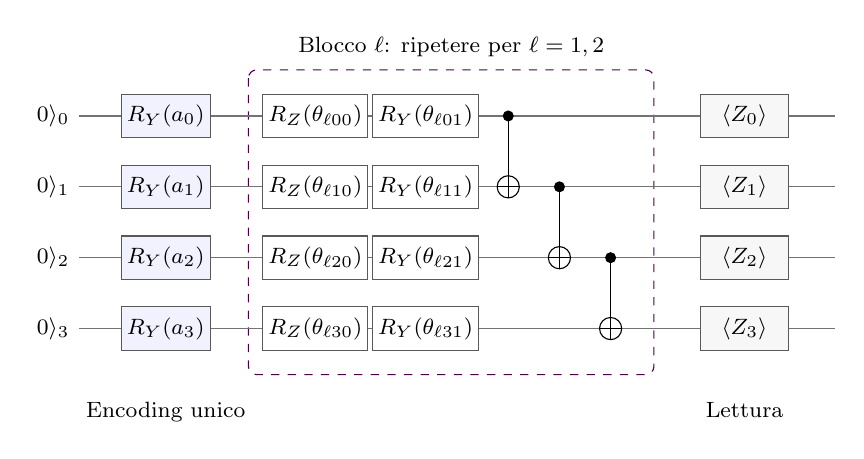
\begin{tikzpicture}[
  x=1cm,y=0.9cm,font=\footnotesize,
  gate/.style={draw=black!65,fill=white,minimum height=0.55cm,
    minimum width=1.12cm,inner sep=2pt}
]
\draw[dashed,rounded corners=3pt,draw=violet!60!black]
  (2.15,0.65) rectangle (7.3,-3.65);
\node[anchor=south,align=center] at (4.725,0.7)
  {Blocco \(\ell\): ripetere per \(\ell=1,2\)};
\foreach \j in {0,1,2,3}{
  \draw[black!55] (0,-\j) -- (9.6,-\j);
  \node[anchor=east] at (0,-\j) {\(\lvert0\rangle_{\j}\)};
  \node[gate,fill=blue!5] at (1.1,-\j) {\(R_Y(a_{\j})\)};
  \node[gate] at (3,-\j) {\(R_Z(\theta_{\ell\j0})\)};
  \node[gate] at (4.4,-\j) {\(R_Y(\theta_{\ell\j1})\)};
  \node[gate,fill=black!3] at (8.45,-\j) {\(\langle Z_{\j}\rangle\)};
}
\foreach \x/\control/\target in {5.45/0/1,6.1/1/2,6.75/2/3}{
  \draw (\x,-\control) -- (\x,-\target);
  \fill (\x,-\control) circle (2pt);
  \draw[fill=white] (\x,-\target) circle (4pt);
  \draw (\x-0.14,-\target) -- (\x+0.14,-\target);
  \draw (\x,-\target-0.155) -- (\x,-\target+0.155);
}
\node[anchor=north] at (1.1,-3.9) {Encoding unico};
\node[anchor=north] at (8.45,-3.9) {Lettura};
\end{tikzpicture}

\caption{Circuito a quattro qubit. L'encoding \(R_Y(a_j)\) viene
eseguito una volta; il riquadro tratteggiato viene ripetuto due volte,
con parametri diversi nei due blocchi. Le CNOT formano una catena
aperta nell'ordine da sinistra a destra. L'uscita comprende i quattro
valori attesi locali di Pauli-\(Z\).}
\label{fig:circuito-q4}
\end{figure}

Il tensore variazionale ha forma \(L\times q\times2\), per un totale
di \(2Lq\) parametri: \(16\) con quattro qubit e \(32\) con otto.
Il numero di CNOT è \(L(q-1)\), rispettivamente \(6\) e \(14\).
La dimensione dello spazio di Hilbert passa da \(2^4=16\) a
\(2^8=256\), ma questi numeri non indicano né il numero di immagini
memorizzabili né il numero di feature classiche indipendenti fornite
all'encoding. La crescita dello spazio degli stati non costituisce,
da sola, una garanzia di capacità utile o di generalizzazione.

\subsection{Lettura e classificazione}

Dal circuito vengono estratti i valori attesi
\begin{equation}
  z_j=
  \langle\psi(\boldsymbol a,\boldsymbol\theta)|
     Z_j|\psi(\boldsymbol a,\boldsymbol\theta)\rangle,
  \qquad j=0,\ldots,q-1.
  \label{eq:lettura-z}
\end{equation}
Il vettore \(\boldsymbol z\in[-1,1]^q\) alimenta un classificatore affine:
\[
  \boldsymbol\ell_{\mathrm Q}
    =W_{\mathrm{out}}\boldsymbol z+\boldsymbol b_{\mathrm{out}}.
\]
Le probabilità di classe derivano dalla softmax, non direttamente dalla
misura di un singolo qubit. In particolare, gli otto qubit della variante
più grande non corrispondono a otto classi.

\subsection{QF: circuito congelato, rete ancora addestrabile}
\label{sec:qf}

QF ha la stessa espressione di Q, ma il tensore
\(\boldsymbol\theta\) resta fisso ai valori iniziali. Proiezione
\(W_{\mathrm{in}},\boldsymbol b_{\mathrm{in}}\) e classificatore
\(W_{\mathrm{out}},\boldsymbol b_{\mathrm{out}}\) rimangono addestrabili.
Il circuito continua quindi a elaborare input che cambiano durante
l'ottimizzazione.

Congelare i pesi non interrompe il gradiente rispetto agli angoli.
La regola della catena contiene infatti il contributo
\[
  \frac{\partial\mathcal L}{\partial W_{\mathrm{in}}}
  =\frac{\partial\mathcal L}{\partial\boldsymbol z}
    \frac{\partial\boldsymbol z}{\partial\boldsymbol a}
    \frac{\partial\boldsymbol a}{\partial W_{\mathrm{in}}},
\]
che deve essere calcolato anche in QF. Non è pertanto corretto attendersi
che il costo del circuito congelato scompaia. L'implementazione esclude
i pesi quantistici dall'ottimizzatore e ne controlla il checksum durante
il training.

Il confronto Q--QF valuta il beneficio dell'ottimizzazione circuitale
all'interno di questo sistema congiunto. Non isola invece l'effetto
dell'entanglement: entrambi i modelli contengono le stesse CNOT.

\subsection{Passaggi essenziali dell'implementazione}
\label{sec:snippet-reti}

I listati seguenti collegano la descrizione matematica al codice
effettivamente utilizzato. Sono estratti dei moduli
\texttt{models/classical.py} e \texttt{models/pennylane\_qnn.py}
del package \texttt{tesi\_qml}, con ritorni a capo adattati alla pagina.
Non sono programmi autonomi: import, costruttori e gestione dei dati
sono omessi. In particolare, \texttt{scale\_angles} applica
\(\pi\tanh\) nella configurazione degli esperimenti.

Il ramo attivo della funzione \texttt{scale\_angles} e la proiezione
del costruttore sono riportati nel \cref{lst:angle-projection}.
I frammenti appartengono a due punti distinti del codice; gli altri
modi di scaling, non usati nel confronto, sono omessi.

\begin{code}
\begin{minted}{python}
# Costruttore di PennylaneAngleQNN
self.pre_quantum = nn.Linear(input_dim, n_qubits)

# Ramo di scale_angles usato negli esperimenti
if mode == "tanh_pi":
    return torch.tanh(values) * math.pi
\end{minted}
\caption{Proiezione da 512 feature a \(q\) componenti e conversione
in angoli. Commenti aggiunti per distinguere i due estratti.}
\label{lst:angle-projection}
\end{code}

\begin{code}
\begin{minted}{python}
def forward(self, features: torch.Tensor) -> torch.Tensor:
    latent = scale_angles(
        self.pre_head(features), self.angle_scale
    )
    return self.classifier(latent)
\end{minted}
\caption{Forward del controllo classico B2.}
\label{lst:b2-forward}
\end{code}

Il \cref{lst:b2-forward} rende esplicito che B2 usa direttamente il
vettore compresso per classificare. Nel modello Q, invece, il medesimo
tipo di proiezione produce gli angoli di ingresso del circuito.

\begin{code}
\begin{minted}{python}
def forward(self, features: torch.Tensor) -> torch.Tensor:
    angles = scale_angles(
        self.pre_quantum(features), self.angle_scale
    )
    quantum_features = self.quantum_layer(angles).to(
        dtype=features.dtype
    )
    return self.post_quantum(quantum_features)
\end{minted}
\caption{Forward della testa ibrida, condiviso da Q e QF.}
\label{lst:q-forward}
\end{code}

Il circuito richiamato dal \cref{lst:q-forward} è definito mediante
un QNode PennyLane. Nella matrice principale \texttt{diff\_method}
è \texttt{backprop}, \texttt{spec.n\_layers} vale due e
\texttt{spec.entangling\_pairs} contiene le coppie adiacenti
\((0,1),\ldots,(q-2,q-1)\), nell'ordine indicato.

\begin{code}
\begin{minted}{python}
@qml.qnode(device, interface="torch", diff_method=diff_method)
def circuit(inputs, weights):
    for wire in range(spec.n_qubits):
        qml.RY(inputs[..., wire], wires=wire)
    for layer in range(spec.n_layers):
        for wire in range(spec.n_qubits):
            qml.RZ(weights[layer, wire, 0], wires=wire)
            qml.RY(weights[layer, wire, 1], wires=wire)
        for control, target in spec.entangling_pairs:
            qml.CNOT(wires=[control, target])
    return [
        qml.expval(qml.PauliZ(wire))
        for wire in range(spec.n_qubits)
    ]
\end{minted}
\caption{Encoding singolo, strati variazionali e lettura del circuito.}
\label{lst:q-circuit}
\end{code}

L'encoding è esterno al ciclo sugli strati: il listato documenta
quindi l'assenza di data re-uploading. La lettura restituisce un valore
atteso per qubit, successivamente trasformato nei logit dal livello
\texttt{post\_quantum}.

\begin{code}
\begin{minted}{python}
self.quantum_weight().requires_grad_(not self.quantum_frozen)
\end{minted}
\caption{Controllo dell'addestrabilità dei soli pesi circuitali.}
\label{lst:qf-freeze}
\end{code}

Il metodo \texttt{quantum\_weight()} restituisce il tensore
\texttt{self.quantum\_layer.weights}. Il flag
\texttt{quantum\_frozen} vale \texttt{False} in Q e \texttt{True}
in QF. Il \cref{lst:qf-freeze} modifica soltanto l'addestrabilità
di quel tensore, non quella dei livelli classici. Il forward del
circuito non è racchiuso in \texttt{torch.no\_grad()}: tale scelta
interromperebbe anche il percorso necessario ad addestrare la
proiezione iniziale.

\section{Numero di parametri e controlli di appaiamento}
\label{sec:capacita-appaiamento}

\subsection{Capacità comparabile, non equivalenza architetturale}

I parametri delle due trasformazioni affini condivise sono
\begin{equation}
  P_{\mathrm{cl}}(q,K)=(512+1)q+(q+1)K.
\end{equation}
B2 ottimizza \(P_{\mathrm{cl}}\) parametri; Q ne ottimizza
\(P_{\mathrm{cl}}+2Lq\). QF conserva lo stesso numero totale di parametri
di Q, ma ne ottimizza soltanto \(P_{\mathrm{cl}}\).
I conteggi nella \cref{tab:parametri-modelli}, verificati rispetto
alle metriche delle run, escludono il backbone congelato condiviso.

\begin{table}[tbp]
\centering
\caption{Parametri delle teste di classificazione. Ogni cella riporta
totali/addestrabili; in QF la differenza corrisponde ai pesi circuitali
congelati. Il backbone non è incluso.}
\label{tab:parametri-modelli}
\begin{tabular}{lrr}
\toprule
\rowcolor{ThesisTableHeader}
\tablehead{Configurazione} & \tablehead{Binario (\(K=2\))} & \tablehead{Tre classi (\(K=3\))} \\
\midrule
B0 & \(1\,026/1\,026\) & \(1\,539/1\,539\)\\
B1 & \(263\,682/263\,682\) & \(264\,195/264\,195\)\\
\textbf{B2--4} & \(2\,062/2\,062\) & \(2\,067/2\,067\)\\
\textbf{B2--8} & \(4\,122/4\,122\) & \(4\,131/4\,131\)\\
\textbf{Q--4} & \(2\,078/2\,078\) & \(2\,083/2\,083\)\\
\textbf{Q--8} & \(4\,154/4\,154\) & \(4\,163/4\,163\)\\
QF--4 & \(2\,078/2\,062\) & \(2\,083/2\,067\)\\
QF--8 & \(4\,154/4\,122\) & \(4\,163/4\,131\)\\
\bottomrule
\end{tabular}
\end{table}

La maggior parte dei parametri delle teste ibride appartiene dunque
agli strati classici. L'espressione \emph{capacity-matched} viene
utilizzata in senso operativo: stessa dimensione di compressione,
stesse interfacce affini e numero di parametri vicino. Non implica
uguaglianza delle classi di funzioni realizzabili, della geometria
dell'ottimizzazione o della capacità statistica.

Inoltre, passare da quattro a otto qubit modifica anche le dimensioni
degli strati classici. Il confronto \(8-4\) non misura quindi un effetto
del solo registro quantistico a parità di tutti gli altri parametri.
B2 nelle due dimensioni fornisce il riferimento per interpretare
questa variazione.

\subsection{Inizializzazione e sorgenti di casualità}

Per ciascun task, repeat seed e dimensione \(q\), B2, Q e QF iniziano
con gli stessi pesi e bias della proiezione e del classificatore.
Le componenti di uno strato affine con \(d\) ingressi sono estratte
uniformemente in \([-1/\sqrt d,1/\sqrt d]\). Q e QF condividono anche
i pesi circuitali iniziali, estratti da
\[
  \theta_{\ell jr}\sim\mathcal N(0,0{,}05^2).
\]
Dopo l'inizializzazione, le reti vengono addestrate separatamente:
l'appaiamento non impone che i pesi classici restino uguali.

Il repeat seed determina sotto-seed distinti per vista delle feature,
inizializzazione condivisa, inizializzazione quantistica, ordine del
DataLoader e librerie. L'ordine degli esempi è condiviso tra B2, Q e QF;
le selezioni dei subset usano lo stesso insieme di oggetti.
Negli artefatti finali, i \(160\) gruppi definiti da
task, regime, dimensione e seed presentano metadati coerenti per
questi controlli e per i checksum iniziali.

L'inizializzazione a piccoli angoli è una scelta del protocollo, non
una dimostrazione di assenza di \emph{barren plateau}. Il fenomeno
discusso da McClean et al.~\cite{mcclean2018barren} riguarda la
concentrazione dei gradienti in determinate famiglie di circuiti.
Per diagnosticarlo qui servirebbero misure specifiche dei gradienti
circuitali e della loro dipendenza dalla dimensione, non la sola
presenza di un training concluso.

\section{Addestramento e selezione del modello}
\label{sec:addestramento}

\subsection{Funzione obiettivo e ottimizzatore}

Tutte le teste minimizzano la cross-entropy non pesata:
\begin{equation}
  \mathcal L=-\frac{1}{B}\sum_{i=1}^{B}\log p_{i,y_i},
  \label{eq:crossentropy}
\end{equation}
dove \(B\) è il numero di esempi nel minibatch. La funzione
\texttt{CrossEntropyLoss} riceve direttamente i logit, evitando
un'applicazione preventiva della softmax nella funzione di costo.

L'ottimizzatore è AdamW, con learning rate iniziale \(10^{-3}\) e
weight decay \(10^{-4}\). AdamW separa il decadimento dei pesi
dall'aggiornamento adattivo dovuto al gradiente
\cite{loshchilov2019adamw}; non viene quindi descritto come la semplice
aggiunta di una penalizzazione \(L_2\) alla loss. L'implementazione
utilizza i valori predefiniti di AdamW per
\(\beta_1=0{,}9\), \(\beta_2=0{,}999\) ed \(\epsilon=10^{-8}\).
Il gradiente complessivo viene limitato con clipping della norma
euclidea a \(1\), prima dell'aggiornamento.

B2, Q e QF utilizzano batch da \(8\) esempi. B0 e B1 impiegano batch
da \(32\): la parità di minibatch riguarda quindi il confronto centrale,
non tutte le baseline. La \cref{tab:training-config} riassume le
condizioni comuni, mantenute anche nei subset.

\begin{table}[tbp]
\centering
\caption{Configurazione di addestramento della matrice finale.
Il learning rate del backbone previsto nel file generale
non è utilizzato, perché il backbone è congelato.}
\label{tab:training-config}
\begin{tabularx}{\textwidth}{@{}lY@{}}
\toprule
\rowcolor{ThesisTableHeader}
\tablehead{Impostazione} & \tablehead{Valore} \\
\midrule
Input della testa & \(512\) feature precalcolate per immagine\\
Batch B2/Q/QF & \(8\)\\
Batch B0/B1 & \(32\)\\
Loss & Cross-entropy non pesata\\
Ottimizzatore & AdamW; learning rate \(10^{-3}\), weight decay \(10^{-4}\)\\
Clipping & Norma euclidea massima \(1\)\\
Epoche massime & \(80\)\\
Early stopping & Validation loss; patience \(12\), min delta \(10^{-4}\)\\
Scheduler & ReduceLROnPlateau; fattore \(0{,}5\), patience \(4\)\\
Circuito & \(q=4\) oppure \(8\); \(L=2\); \(\sigma_{\mathrm{init}}=0{,}05\)\\
Simulazione & \texttt{default.qubit}, \texttt{shots=None}, backpropagation\\
\bottomrule
\end{tabularx}
\end{table}

\subsection{Validation, arresto e checkpoint migliore}

Dopo ogni epoca vengono calcolate loss e metriche sulla validation.
Lo scheduler riduce il learning rate quando la validation loss
non migliora secondo il criterio di plateau. La decisione di arresto
anticipato è gestita separatamente: il contatore delle epoche senza
miglioramento viene azzerato quando la loss scende di oltre \(10^{-4}\)
rispetto al miglior valore riconosciuto dall'early stopping; il training
termina quando il contatore raggiunge \(12\), oppure all'ottantesima epoca.

La selezione di \texttt{best.pt} applica invece il criterio del minimo
strettamente osservato della validation loss, senza la soglia
\texttt{min\_delta}. Una piccola riduzione può quindi aggiornare il
checkpoint migliore senza azzerare il contatore di early stopping.
Questo dettaglio distingue il criterio di selezione da quello di arresto.

Prima della valutazione finale viene ripristinato \texttt{best.pt}.
Il test viene valutato con quel modello; non guida lo scheduler,
l'early stopping o la scelta dell'epoca. Il confronto riguarda dunque
le prestazioni dei modelli selezionati dalla validation, non
necessariamente quelle dell'ultima epoca.

Gli stessi iperparametri rendono il protocollo controllato, ma non
garantiscono che ogni architettura raggiunga la propria prestazione
ottimale dopo una ricerca dedicata. Analogamente, a parità di epoche,
un subset più piccolo produce meno aggiornamenti dell'ottimizzatore.
Le curve low-resource descrivono quindi il comportamento sotto
questo budget e questa regola di arresto, non sotto un numero fisso
di aggiornamenti.

\subsection{Simulazione e differenziazione}

L'integrazione tra circuito e rete usa PennyLane
\cite{bergholm2018pennylane} e l'interfaccia PyTorch
\cite{paszke2019pytorch}. Il backend è
\texttt{default.qubit}, con \texttt{shots=None}: i valori attesi
sono calcolati sullo stato simulato, senza rumore di campionamento
da un numero finito di misure. Non vengono introdotti canali di rumore
hardware e non viene eseguito alcun circuito su QPU.

Con questa configurazione il codice seleziona la differenziazione
\texttt{backprop}. Il gradiente attraversa le operazioni del simulatore
e gli strati classici. Il parameter-shift, che permette di ricavare
derivate circuitali da valutazioni con parametri traslati
\cite{schuld2019gradients}, costituisce un'alternativa
supportata dal codice per altri backend o configurazioni di misura,
ma non è il metodo usato nelle run della matrice finale.

\section{Matrice sperimentale e gerarchia delle analisi}
\label{sec:matrice-esperimenti}

Per ogni task e regime sono presenti le configurazioni B0, B1,
B2--4, B2--8, QF--4, QF--8, Q--4 e Q--8, ciascuna su dieci seed.
La \cref{tab:matrice-esperimenti} distingue l'esperimento Full
dall'estensione low-resource.

\begin{table}[H]
\centering
\caption{Matrice delle run finali. Tutte le run utilizzano
l'assegnazione \texttt{iteration=1} del repeated holdout.
Il regime da \(50\) immagini, pur previsto nel file generale,
non appartiene alla matrice analizzata.}
\label{tab:matrice-esperimenti}
\begin{tabular}{lrrrr}
\toprule
\rowcolor{ThesisTableHeader}
\tablehead{Regime} & \tablehead{Task} & \tablehead{Configurazioni/task} & \tablehead{Seed} & \tablehead{Run} \\
\midrule
Full & 2 & 8 & 10 & 160\\
100 & 2 & 8 & 10 & 160\\
300 & 2 & 8 & 10 & 160\\
900 & 2 & 8 & 10 & 160\\
\midrule
Totale & & & & 640\\
\bottomrule
\end{tabular}
\end{table}

La famiglia primaria comprende quattro confronti Q--B2 sul Full:
due task per due dimensioni. La famiglia secondaria comprende i
dodici confronti Q--B2 ottenuti aggiungendo i tre subset. La correzione
per confronti multipli viene applicata separatamente alle due famiglie.

Q--QF, sensibilità \(8-4\), analisi della classe merger,
calibrazione e costo hanno finalità esplorativa. Si privilegiano
dimensione dell'effetto e intervalli, senza trasformare tutte le
combinazioni di modelli in ulteriori test confermativi.
Questa gerarchia organizza l'analisi della tesi; non viene presentata
come una preregistrazione pubblica di cui non è disponibile documentazione.

\section{Metriche di valutazione}
\label{sec:metriche}

Le \cref{tab:guida-metriche,tab:guida-indicatori} offrono
una guida alla lettura dei risultati. Le metriche predittive
descrivono aspetti diversi del modello; gli indicatori
inferenziali descrivono invece effetti e incertezza.

\begin{table}[tbp]
\centering
\small
\renewcommand{\arraystretch}{1.18}
\caption{Guida alle metriche e ai costi utilizzati nella valutazione.
Le frecce indicano il verso preferibile, a parità delle altre condizioni.
L'ECE dipende dal binning; Brier score e log-loss non misurano soltanto
la calibrazione.}
\label{tab:guida-metriche}
\begin{tabularx}{\textwidth}{@{}p{2.5cm}Yc@{}}
\toprule
\rowcolor{ThesisTableHeader}
\tablehead{Metrica} & \tablehead{Significato} & \tablehead{Verso} \\
\midrule
Accuracy & Quota di esempi classificati correttamente sul totale. & \(\uparrow\) \\
Precision & Per una classe: quota di assegnazioni a quella classe che sono corrette. & \(\uparrow\) \\
Recall & Per una classe: quota dei suoi esempi reali riconosciuta dal modello. & \(\uparrow\) \\
F1 per classe & Media armonica di precision e recall della classe. & \(\uparrow\) \\
Macro-F1 & Media delle F1 con uguale peso alle classi; metrica principale della tesi. & \(\uparrow\) \\
Balanced accuracy & Media dei recall; coincide con l'accuracy quando i supporti delle classi sono uguali. & \(\uparrow\) \\
Log-loss & Penalità sulle probabilità delle classi vere; cresce per errori molto confidenti. & \(\downarrow\) \\
Brier score & Errore quadratico delle probabilità rispetto alle etichette in forma one-hot. & \(\downarrow\) \\
ECE & Discrepanza aggregata tra confidenza e accuratezza, raggruppando le predizioni per fasce di confidenza. & \(\downarrow\) \\
Tempo di training & Somma dei tempi di epoca registrati; esclude la costruzione della cache di feature. & \(\downarrow\) \\
Tempo di test & Tempo di predizione sull'intero test dalle feature; non latenza end-to-end dalle immagini. & \(\downarrow\) \\
\bottomrule
\end{tabularx}
\end{table}

\begin{table}[tbp]
\centering
\small
\renewcommand{\arraystretch}{1.2}
\caption{Indicatori statistici: non sono metriche di classificazione.
Gli intervalli sono marginali, mentre Holm corregge i test all'interno
delle famiglie definite dal protocollo.}
\label{tab:guida-indicatori}
\begin{tabularx}{\textwidth}{@{}p{2.5cm}Y@{}}
\toprule
\rowcolor{ThesisTableHeader}
\tablehead{Indicatore} & \tablehead{Interpretazione} \\
\midrule
\(\Delta\) Q--B2 & Differenza media appaiata di Macro-F1. Positiva favorisce Q,
negativa B2; è espressa in punti percentuali. \\
IC95\% & Intervallo bootstrap per la quantità stimata, come media o differenza.
Non è l'intervallo che contiene il 95\% delle run. \\
\(p_{\mathrm{Holm}}\) & P-value corretto per i confronti multipli della famiglia.
Non è la probabilità che l'ipotesi nulla sia vera, né misura l'ampiezza dell'effetto. \\
\(d_z\) & Differenza media divisa per la deviazione standard delle differenze
appaiate: misura standardizzata dell'effetto. \\
\bottomrule
\end{tabularx}
\end{table}


\subsection{Macro-F1 e metriche per classe}

La metrica principale è la Macro-F1. Per la classe \(c\), indicando con
\(\mathrm{TP}_c\), \(\mathrm{FP}_c\) e \(\mathrm{FN}_c\) veri positivi,
falsi positivi e falsi negativi,
\begin{equation}
 F_{1,c}=\frac{2\mathrm{TP}_c}
 {2\mathrm{TP}_c+\mathrm{FP}_c+\mathrm{FN}_c},
 \qquad
 F_{1,\mathrm{macro}}=\frac{1}{K}\sum_{c=1}^{K}F_{1,c}.
\end{equation}
Le classi ricevono uguale peso: si usa la media delle F1 per classe,
coerentemente con \texttt{average='macro'} di scikit-learn
\cite{sklearn17f1}, non la media armonica di precision e recall macro.
Vengono inoltre conservate accuracy,
balanced accuracy, precision e recall, sia aggregate sia per classe.
Per i merger, precision, recall e F1 sono riportate separatamente
per distinguere le diverse modalità di errore.

La matrice di confusione normalizzata per riga descrive la distribuzione
delle predizioni condizionata alla classe reale. Per il confronto tra
architetture, la sintesi viene effettuata a livello di seed, evitando
di interpretare la somma dei test parzialmente sovrapposti come un
unico campione indipendente.

Le metriche ROC sono calcolate in modalità one-vs-rest. Il campo
\texttt{pr\_auc} degli artefatti è ottenuto con
\texttt{average\_precision\_score}: è quindi \emph{average precision},
non l'area trapezoidale generica sotto una curva precision--recall
\cite{sklearn17averageprecision}.
Il nome del campo va quindi distinto dalla definizione della metrica.

\subsection{Qualità delle probabilità}

La calibrazione riguarda la corrispondenza tra confidenza prevista
e frequenza di correttezza, e non coincide con la sola accuratezza
\cite{guo2017calibration}. L'analisi conserva log-loss, Brier score
ed expected calibration error (ECE).

Brier score e log-loss valutano la distribuzione di probabilità
assegnata alle classi, non soltanto la confidenza della decisione
finale. Appartengono alla famiglia delle scoring rule proprie
\cite{gneiting2007scoring}; non sono quindi errori di sola calibrazione.

Il Brier score multiclasse viene calcolato come
\begin{equation}
  \mathrm{BS}=\frac{1}{N}\sum_{i=1}^{N}\sum_{c=1}^{K}
     \left(p_{ic}-\mathbf 1\{y_i=c\}\right)^2.
\end{equation}
La somma sulle classi non viene ulteriormente divisa per \(K\).
L'ECE usa \(15\) intervalli equidistanti della confidenza massima:
\[
 \mathrm{ECE}=\sum_{b=1}^{15}
 \frac{|I_b|}{N}
 \left|\mathrm{acc}(I_b)-\mathrm{conf}(I_b)\right|.
\]
Il risultato dipende dalla discretizzazione e dalla numerosità del
campione. Queste metriche sono diagnostiche complementari; non è
stato applicato un ricalibratore post-hoc. Nei confronti Q--B2,
una differenza positiva di tali errori favorisce B2, diversamente
dalla convenzione usata per la Macro-F1.

\section{Confronti appaiati e incertezza}
\label{sec:statistica}

\subsection{Unità di analisi e differenza media}

Per task, regime e dimensione fissati si definisce, per ciascun seed \(s\),
\begin{equation}
  d_s=F^{\mathrm Q}_{1,\mathrm{macro},s}
      -F^{\mathrm{B2}}_{1,\mathrm{macro},s},
  \qquad
  \overline d=\frac{1}{10}\sum_{s=1}^{10}d_s.
  \label{eq:delta-appaiato}
\end{equation}
Valori positivi favoriscono Q. Le differenze mostrate nei grafici
sono \(100d_s\), espresse in punti percentuali: una differenza di
\(0{,}01\) in Macro-F1 equivale a un punto percentuale, non a un
incremento relativo dell'uno per cento.

La ripetizione identificata dal seed costituisce l'unità di
ricampionamento. I risultati dei modelli vengono abbinati prima
di calcolare differenze e intervalli. La differenza delle medie
coincide con la media delle differenze, ma l'incertezza va stimata
ricampionando le coppie: trattare le due serie come indipendenti
perderebbe la struttura dell'appaiamento.

\subsection{Bootstrap e intervalli al 95\%}

L'\cref{app:codice-appaiamento} riporta il nucleo implementativo
dell'appaiamento e del bootstrap, separando la costruzione delle
coppie dal ricampionamento delle differenze.

La procedura bootstrap ricampiona con reinserimento le dieci
osservazioni per seed e ricalcola la statistica
\cite{efron1979bootstrap}. Si utilizzano \(10\,000\) ricampionamenti
e i quantili \(2{,}5\%\) e \(97{,}5\%\) delle statistiche ricampionate.
Per la Macro-F1 e per gli effetti appaiati la statistica è la media;
per le sintesi dei rapporti di costo viene usata la mediana.

Gli intervalli dei grafici finali sono bootstrap percentile,
non intervalli di predizione per una nuova galassia e non intervalli
simultanei corretti per tutti i confronti. Alcuni riepiloghi intermedi
del progetto usano intervalli basati sulla distribuzione \(t\):
sono distinti da quelli ricalcolati per le figure finali.
Anche due intervalli bootstrap dello stesso effetto possono differire
leggermente se ottenuti con seed di ricampionamento diversi.

\subsection{Test sign-flip e correzione di Holm}

Per Q--B2 viene utilizzato un test bilaterale sign-flip sulla media
delle differenze. Ogni replica genera segni
\(\varepsilon_s\in\{-1,+1\}\) e calcola
\[
  T^*=\left|\frac{1}{10}\sum_{s=1}^{10}\varepsilon_s d_s\right|,
  \qquad T_{\mathrm{obs}}=|\overline d|.
\]
Con \(R=10\,000\) repliche Monte Carlo, il p-value è
\begin{equation}
  p=\frac{1+\sum_{r=1}^{R}\mathbf 1\{T_r^*\ge T_{\mathrm{obs}}\}}{R+1}.
\end{equation}
Con dieci coppie esistono soltanto \(2^{10}=1\,024\) combinazioni
distinte di segni: il codice le campiona con ripetizione, non effettua
un'enumerazione esatta. Il numero di repliche non aumenta quindi il
numero di unità sperimentali.

I p-value sono corretti con la procedura step-down di Holm
\cite{holm1979multiple}, separatamente per i quattro test primari
e i dodici secondari. La soglia adottata è
\(p_{\mathrm{Holm}}<0{,}05\). Gli artefatti riportano anche il test
di Wilcoxon e la dimensione standardizzata
\(d_z=\overline d/s_d\), dove \(s_d\) è la deviazione standard
campionaria delle differenze; tali quantità sono complementari,
non criteri alternativi tra cui scegliere quello più favorevole.

Come richiamato nel \cref{chap:dataset}, le ripetizioni condividono
il dataset. Il bootstrap semplice sui seed e il sign-flip non
modellano esplicitamente la dipendenza dovuta agli holdout
sovrapposti. Il problema di stimare l'incertezza tenendo conto sia
del training sia del test è discusso da Nadeau e Bengio
\cite{nadeau2003inference}; la presente analisi non applica il loro
stimatore corretto della varianza. Inoltre il sign-flip richiede
un'appropriata simmetria
sotto l'ipotesi nulla, non la sola uguaglianza delle medie.
Gli intervalli e i p-value vengono pertanto interpretati nel perimetro
del protocollo, senza attribuire loro una validità incondizionata
sulla popolazione astronomica. Holm tratta la molteplicità dei test,
non corregge queste assunzioni dei test di partenza.
L'assenza di significatività non dimostra equivalenza tra modelli.

\subsection{Analisi esplorative tra task e architetture}

Per confrontare il passaggio dal binario alle tre classi viene calcolata,
entro ciascun seed e a parità di regime e dimensione, la
differenza-in-differenze
\begin{equation}
 D_s=
 \left(F^{\mathrm Q}_{1,s}-F^{\mathrm{B2}}_{1,s}\right)_{\mathrm{tre}}
 -
 \left(F^{\mathrm Q}_{1,s}-F^{\mathrm{B2}}_{1,s}\right)_{\mathrm{binario}}.
 \label{eq:did}
\end{equation}
Un valore negativo indica che Q perde terreno rispetto a B2 nel task
a tre classi. È un contrasto descrittivo appaiato, non una stima causale:
cambiano numero di classi, composizione del problema e, nel Full,
anche numerosità totale del training.

Analogamente vengono costruite le differenze Q--QF e \(8-4\),
ricampionando i contrasti per seed. Le analisi merger e calibrazione
completano la lettura delle prestazioni senza introdurre nuove
famiglie di test oltre a quelle primaria e secondaria.

\section{Costo computazionale e riproducibilità}
\label{sec:costo-riproducibilita}

\subsection{Che cosa misurano i tempi}

Il campo \texttt{training\_seconds} è la somma dei tempi di epoca
registrati nella history. Comprende training, validation e calcolo
delle metriche interne all'epoca, ma non la costruzione iniziale della
cache di feature, la valutazione finale e il successivo salvataggio
dei checkpoint o dell'archivio. Non coincide quindi con il tempo
trascorso dall'avvio della sessione Colab alla sua chiusura.

Il tempo di predizione riportato nel capitolo dei risultati è
\texttt{test\_inference\_seconds}: misura la predizione sull'intero
test, a partire dalle feature, dopo il ripristino del checkpoint
migliore. È distinto da \texttt{inference\_seconds}, che negli
artefatti misura la predizione sulla validation. Le metriche
predittive sono quelle di \texttt{test\_metrics.json}.
Questi tempi non misurano una latenza end-to-end dall'immagine,
né il solo tempo di esecuzione delle porte quantistiche.

I rapporti di costo vengono calcolati per seed, per esempio
\(t_{\mathrm Q,s}/t_{\mathrm{B2},s}\), e poi sintetizzati con la mediana.
Il rapporto delle mediane non è, in generale, la stessa quantità.
Nella figura prestazioni--costo ogni configurazione è rappresentata
invece dalla Macro-F1 media e dal tempo di training mediano.

\subsection{Ambienti effettivi e comparabilità dei regimi}
\label{sec:ambiente-hardware}

I confronti temporali sono effettuati entro ciascun regime, nel quale
i modelli appaiati condividono il dispositivo di esecuzione. Full è
stato eseguito su GPU Tesla T4 e i subset su CPU; i tempi tra regimi
diversi non sono pertanto interpretati come una misura di scaling
a hardware costante. Anche il confronto predittivo tra subset e Full
non mantiene identico l'ambiente numerico, pur conservando le
partizioni e gli iperparametri previsti dal protocollo.

Le versioni riportate dalle run sono sintetizzate nella
\cref{tab:ambiente-run}. I tempi rimangono misure empiriche di una
simulazione classica in Colab, condizionate anche da carico della
macchina, trasferimenti e overhead software: non forniscono una
stima dello speed-up ottenibile su hardware quantistico.

\begin{table}[tbp]
\centering
\caption{Versioni software dichiarate nei metadati delle run finali.
Il backend quantistico è \texttt{default.qubit}; la versione CUDA
si riferisce alla build software, non al dispositivo usato da ogni run.}
\label{tab:ambiente-run}
\begin{tabular}{ll}
\toprule
\rowcolor{ThesisTableHeader}
\tablehead{Componente} & \tablehead{Versione} \\
\midrule
Python & 3.13.15\\
PyTorch / TorchVision & 2.8.0 / 0.23.0\\
PennyLane & 0.42.3\\
NumPy / pandas & 2.2.6 / 2.3.3\\
scikit-learn & 1.7.2\\
CUDA dichiarata dalla build & 12.8\\
\bottomrule
\end{tabular}
\end{table}

\subsection{Artefatti e limiti delle diagnostiche}

Ogni run conserva configurazione, fingerprint, storia delle epoche,
checkpoint migliore e ultimo checkpoint, metriche e predizioni.
La ripresa controlla l'identità della configurazione e ripristina
anche stato dell'ottimizzatore, scheduler e sorgenti di casualità.
Questi meccanismi supportano la tracciabilità delle esecuzioni
interrotte, ma non rendono intercambiabili ambienti software diversi.

L'audit distingue inoltre il nome di una diagnostica dalla quantità
realmente calcolata. Nella versione usata, il filtro della
\texttt{quantum\_gradient\_norm} seleziona i parametri il cui nome
contiene la parola \texttt{quantum}; include quindi anche
\texttt{pre\_quantum} e \texttt{post\_quantum}. Quel campo non isola
i soli angoli variazionali e non viene utilizzato per sostenere
conclusioni sull'assenza di barren plateau.

Con queste precisazioni, il disegno sperimentale consente di valutare
prestazioni, stabilità e costo relativo delle teste sotto condizioni
documentate. Il capitolo successivo presenta gli effetti osservati;
l'attribuzione di eventuali differenze a specifici meccanismi fisici
o di ottimizzazione resta invece materia di discussione e di ulteriori
esperimenti.
